\section{Amostras e Análise de Dados}
Com os textos devidamente pré-processados e com os atributos selecionados, é necessário a coleta de uma amostra para que seja possível em uma segunda parte do processo, adicionar os atributos referentes a futura inferência da EADS, para que essa amostra seja coletada é necessário que em primeiro instante seja feita uma análise dos dados. Para entender a próxima análise é necessário compreender que a análise de sentimento retorna dois fatores: score e magnitude, o score varia entre 1 e -1, sendo 1 representativo ao sentimento positivo e -1 o negativo, logo 0 seria neutro. Além disso existe a magnitude que é para expressar o quão o sentimento é presente no texto. 

No caso do Twitter (280 caracteres máximos) por postagem as pessoas tendem a ser mais diretas e sucintas, logo a magnitude é muito variável e pode ser um dado que venha a confundir em vez de ajudar, logo, foi agrupado os tweets pelos scores, a cada espaçamento de 0.2. Ao observar o Figura \ref{fig:sentiment-relation}, notasse que as extremidades tendem a ter menos tweets, média de 1000 a 2500 tweets por agrupamento, entretanto grupos mais centralizados (emoções neutras) chegam a picos de 8104 tweets, já que o dado desejado é uma massa negativa e seus usuários será dado enfoque ao lado negativo do mapeamento.

\begin{figure}
    \centering
    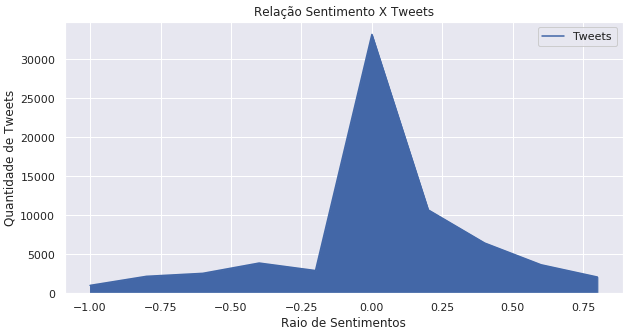
\includegraphics[width=.4\textwidth]{imagens/relacao-sentimento.png}
    \caption{Relação de sentimentos por tweet dentro da massa de dados}
    \label{fig:sentiment-relation}
\end{figure}


Partindo do principio que a partir de um score de -0.2 já existem menos dados, foi tomada como premissa que qualquer dado com score superior a esse é um dado não viável para amostra. Seguindo essa premissa é preciso mapear de cada usuário o percentual de publicações a abaixo de -0.2, com isso será possível obter um percentual da densidade de publicações negativas naquele perfil. Analisando os dados da Figura \ref{fig:negative-pop-relation}, é possível notar que a maior quantidade de percentual negativo esta entre 20\% e 40\%, entretanto, é impossível afirmar que os dados suprem as necessidades que a inteligência artificial ira necessitar para realizar a inferência na base. Refletindo sobre a EADS, a versão minificada tem 21 perguntas, logo, necessita-se de no mínimo 21 tweets negativos na esperança que cada um responda pelo menos 1 das perguntas. Para validar a ideia é necessário descobrir a média de tweets dentro dos percentuais que mais contem massa negativa.

\begin{figure}[!h]
    \centering
    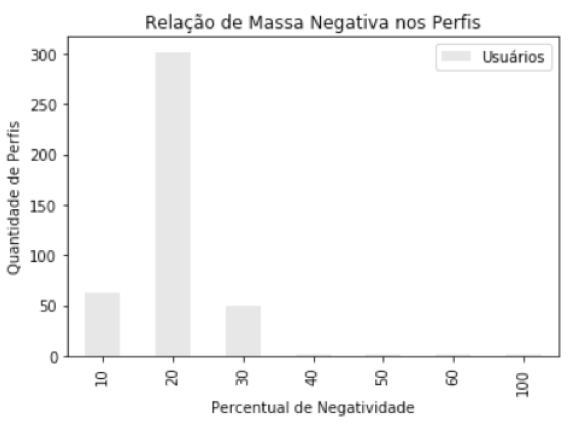
\includegraphics[width=.4\textwidth]{imagens/relacao-massa-neg.png}
    \caption{Percentual de massa negativa por quantidade de perfis}
    \label{fig:negative-pop-relation}
\end{figure}

Entretanto, pode-se notar mais um fator no dado, existem perfis com 100\% de sentimento negativo devido a conter um único tweet negativo, ou seja, a quantidade de tweets é algo relevante. Logo foi feito uma cáculo a partir dos dados retirados, a quantidade de tweets negativos entre 20\% a 40\% de massa negativa é equivalente a 9592, de um total de 413 usuários, a média retirada foi de aproximadamente 23 tweets negativos por usuário da massa.

Uma vez obtido os dados do percentual e média de tweets é possível configurar o script para gerar amostra. Como dito são 21 questões, que representam o total de questões da EADS, logo, é necessário um mínimo de 21 tweets negativos (já contemplado pela média de 23), logo para aumentar a eficácia uma nova média foi retirada do dobro de questões somado a média atual de tweets negativos, o que deu aproximadamente 32 tweets. Dessa amostra foram minerados 21 perfis e 907 tweets negativos. Se observar as Figura \ref{fig:sample-relation} é possível notar que a média de tweets negativos pegos para análise em relação a base é de 1.3\% enquanto em relação aos usuários 5\%.

\begin{figure}[!h]
    \centering
    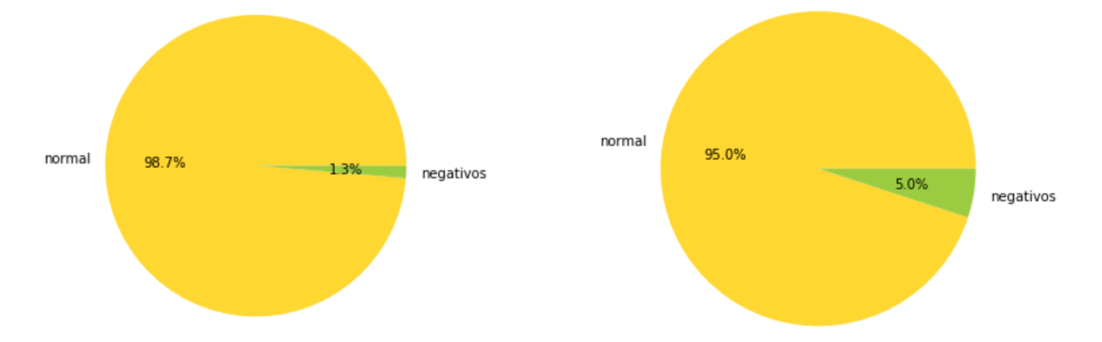
\includegraphics[width=.6\textwidth]{imagens/relacao-amostra.png}
    \caption{Percentual de dados utilizados na amostra em relação a base total de tweets e usuários}
    \label{fig:sample-relation}
\end{figure}

